%% ****** Start of file template.aps ****** %
%%
%%
%%   This file is part of the APS files in the REVTeX 4 distribution.
%%   Version 4.0 of REVTeX, August 2001
%%
%%
%%   Copyright (c) 2001 The American Physical Society.
%%
%%   See the REVTeX 4 README file for restrictions and more information.
%%
%
% This is a template for producing manuscripts for use with REVTEX 4.0
% Copy this file to another name and then work on that file.
% That way, you always have this original template file to use.
%
% Group addresses by affiliation; use superscriptaddress for long
% author lists, or if there are many overlapping affiliations.
% For Phys. Rev. appearance, change preprint to twocolumn.
% Choose pra, prb, prc, prd, pre, prl, prstab, or rmp for journal
%  Add 'draft' option to mark overfull boxes with black boxes
%  Add 'showpacs' option to make PACS codes appear

%\RequirePackage{lineno}

 \documentclass[aps,prl,twocolumn,showpacs,superscriptaddress,groupedaddress]{revtex4}  % for review and submission
\usepackage{graphicx}  % needed for figures
\usepackage{dcolumn}   % needed for some tables
\usepackage{bm}        % for math
\usepackage{amssymb}   % for math
\usepackage{amsmath}
\usepackage{color}
\usepackage{multirow}
 \usepackage{rotating}
\usepackage{xspace}
\usepackage{comment}
\usepackage{slashed}


\pagenumbering{arabic}
\renewcommand{\thetable}{\Roman{table}}


%---------------------------------------------------------------------

% avoids incorrect hyphenation
\hyphenation{ALPGEN}
\hyphenation{EVTGEN}
\hyphenation{PYTHIA}

\newcommand{\fix}[1]{} % comment this in if you want to the see the PRL without comments
\newcommand{\MET}{\mbox{$\raisebox{.3ex}{$\not\!$}E_T$}}
\newcommand{\METVEC}{\mbox{$\raisebox{.3ex}{$\not\!$}{\vec E}_T$}}
\newcommand{\MPTVEC}{\mbox{$\raisebox{.3ex}{$\not\!$}{\vec {p}_T}$}}
\def\DZero{D0~}



%%%% MET +JETS %$$$$$$$$$
\newcommand{\Et}{\mbox{$E_T$}}
\newcommand{\Pt}{\mbox{$p_T$}}
\newcommand{\Ht}{\mbox{$H_T$}}
\newcommand{\met}{\mbox{$\protect \raisebox{0.3ex}{$\not$}\Et$}}
\newcommand{\mpt}{\mbox{$\protect \raisebox{0.3ex}{$\not$}\Pt$}}

\newcommand{\rar}       {\rightarrow}
\newcommand{\rargap}    {\mbox{ $\rightarrow$ }}
\newcommand{\pt} {\mbox{$p_T$}}
\newcommand{\dzero}     {D0}
\newcommand{\ttbar}     {\mbox{$t\bar{t}$}\xspace}
\newcommand{\bbbar}     {\mbox{$b\bar{b}$}\xspace}
\newcommand{\ccbar}     {\mbox{$c\bar{c}$}\xspace}
\newcommand{\ppbar}     {\mbox{$p\bar{p}$}\xspace}
\newcommand{\ljets}     {\mbox{$\ell$+jets}\xspace}
\newcommand{\comphep}   {\sc comphep}
\newcommand{\singletop} {\sc singletop}
\newcommand{\pythia}    {\mbox{\textsc{pythia}}}
\newcommand{\herwig}    {\mbox{\textsc{herwig}}}
\newcommand{\geant}     {{\sc{geant}}}
\newcommand{\alpgen}    {\mbox{\textsc{alpgen}}}
\newcommand{\mcfm}      {\sc mcfm}
\newcommand{\mcatnlo}   {\mbox{\textsc{mc@nlo}}}
\newcommand{\ifb}       {fb$^{-1}$}

\newcommand{\vtb}   {$|V_{tb}|$}
\newcommand{\Wt}{\ensuremath{\mathit{\!Wt}}\xspace} 

% combined cross section result
\newcommand{\xsectev}{1.29}
\newcommand{\xsecteverrorup}{+0.26}
\newcommand{\xsecteverrordown}{-0.24}


% combined significance result
\newcommand{\probtev}{1.8 \times 10^{-10}}
\newcommand{\sigmatev}{6.3}
\newcommand{\sigmaexp}{5.1}


%---------------------------------------------------------------------


\begin{document}

\hspace{5.2in} \mbox{FERMILAB-PUB-15-088-E}


\title{Tevatron Combination of Single-Top-Quark Cross Sections and
  Determination of the Magnitude of the Cabibbo-Kobayashi-Maskawa
  Matrix Element $\bf V_{tb}$}


%%%%%%%%%%%%%%%%%%%%%%%%%%%
%
\input author.tex  % CDF+D0 author list
%
%%%%%%%%%%%%%%%%%%%%%%%%%%%

\date{January 19, 2016}


\begin{abstract}
\noindent
We present the final combination of CDF and D0 measurements of cross
sections for single-top-quark production in proton-antiproton
collisions at a center-of-mass energy of 1.96~TeV. The data correspond
to total integrated luminosities of  up to 9.7~\ifb\ per
experiment. The $t$-channel cross section is measured to be $\sigma_t
= 2.25^{+0.29}_{-0.31}$~pb. We also present the combinations of the
two-dimensional measurements of the $s$- vs.\ $t$-channel cross
section. In addition, we give the combination of the $s+t$ channel
cross section measurement resulting 
in $\sigma_{s+t} = 3.30^{+0.52}_{-0.40}$~pb, without assuming the
standard-model value for the ratio $\sigma_s/\sigma_t$. The resulting
value of the magnitude of the top-to-bottom quark coupling is
$|V_{tb}|$ = $1.02^{+0.06}_{-0.05}$, corresponding to $|V_{tb}| >
0.92$ at the 95\% C.L.
\end{abstract} 



\pacs{14.65.Ha; 12.15.Ji; 13.85.Qk; 12.15.Hh}
\maketitle

%\modulolinenumbers[1]
%\linenumbers


%---------------------------------------------------------------------




%%%%%%%%%%%%%%%%%%%%%%%%%%%
%% 
%% Introduction
%% 
%%%%%%%%%%%%%%%%%%%%%%%%%%%


The top quark is the heaviest elementary particle of the standard model
(SM). Detailed studies of top-quark production and decay provide
stringent tests of strong and electroweak interactions, as well as
sensitivity to extensions of the SM~\cite{top}. At the Fermilab
Tevatron collider, protons ($p$) and antiprotons ($\bar{p}$) collided
at a center-of-mass energy of $\sqrt{s}=1.96$\;TeV. Top quarks were
produced predominantly in pairs (\ttbar) via the strong
interaction~\cite{ttbar_combi}.  They were also produced singly via
the electroweak interaction. The cross section for single-top-quark
production depends on the square of the magnitude of the quark-mixing 
Cabibbo-Kobayashi-Maskawa (CKM) matrix~\cite{ckm} element $V_{tb}$,
and consequently is sensitive to contributions from a fourth 
family of quarks~\cite{FourthGen1,FourthGen2}, as well as other 
new phenomena~\cite{Tait:2000sh}, which would lead to a measured 
strength of the $Wtb$ coupling $|V_{tb}|$ different from the SM
prediction. Non-SM phenomena could also change the relative fraction
of events produced in the various channels that contribute to the
total single-top-quark production cross section.

In $p{\bar p}$ scattering, single-top-quark production proceeds in the
$t$-channel via the exchange of a spacelike virtual $W$ boson between
a light quark and a bottom
quark~\cite{singletop-willenbrock,singletop-yuan,tchannel-kidonakis}.
Single top quarks are also produced in the $s$ channel via the decay
of a timelike virtual $W$ boson 
produced by quark-antiquark annihilation, which produces a top quark
and a bottom quark~\cite{singletop-cortese}, or in association with a
$W$ boson (\Wt)~\cite{Wt-tait}.  The predicted SM cross section for
the $t$-channel process $\sigma_t$ is $2.10 \pm
0.13$~pb~\cite{tchannel-kidonakis}, while the $s$-channel cross
section $\sigma_s$ is $1.05 \pm 0.06$~pb~\cite{schannel-kidonakis},
both calculated at next-to-leading-order (NLO) in quantum
chromodynamics (QCD), including next-to-next-to-leading logarithmic (NNLL)
corrections. A top-quark mass of 172.5~GeV was chosen, which is
consistent with the 
current world average value~\cite{topmasswa}. The cross section for
\Wt\ production $\sigma_{Wt}$  is negligibly small at the Tevatron and
 therefore is not considered in the combination described in this Letter. 
Since the magnitude of the $Wtb$ coupling is much larger than that of
$Wtd$ or of $Wts$~\cite{pdg}, each top quark decays almost exclusively
to a $W$~boson and a $b$ quark.

Observation of single-top-quark production was reported by the
CDF~\cite{stop-obs-2009-cdf,Aaltonen:2010fs,cdf-prd-2010} and
D0~\cite{stop-obs-2009-d0,stop-2011-d0} Collaborations not
differentiating between
the $s$ and the $t$ channels (hereinafter $s+t$ channel). The CDF
Collaboration subsequently measured a single-top-quark production
cross section for the sum of the $s$, $t$, and \Wt channels of
$\sigma_{s+t+\Wt} =3.04^{+0.57}_{-0.53}$~pb using data corresponding
to 7.5~\ifb\ of integrated luminosity~\cite{cdf_channels_7.5} and for
the sum of the $s$ and $t$ channels of $\sigma_{s+t} =
3.02^{+0.49}_{-0.48}$\;pb using up to 9.5~\ifb\ of integrated
luminosity~\cite{cdf_channels}. The D0 Collaboration obtained
$\sigma_{s+t} = 4.11^{+0.60}_{-0.55}$\;pb using data corresponding to
9.7~\ifb\ of integrated luminosity~\cite{d0_schannel}. 

The cross sections for individual production modes were also measured separately. 
The D0 Collaboration observed the $t$-channel
process~\cite{t-channel-new} and measured its cross section to be $\sigma_t =
3.07^{+0.54}_{-0.49}$\;pb using data corresponding to 9.7~\ifb\ of
integrated luminosity~\cite{d0_schannel}. 
The CDF Collaboration measured $\sigma_{t+\Wt} =
1.66^{+0.53}_{-0.47}$~pb using data corresponding to 7.5~\ifb\ of
integrated luminosity~\cite{cdf_channels_7.5} and $\sigma_t =
1.65^{+0.38}_{-0.36}$\;pb using up to 9.5~\ifb~\cite{cdf_channels} of
integrated luminosity. The difference between the results for
$\sigma_t$ is about 2 standard deviations (s.\ d.). 
Furthermore, both the CDF and D0 Collaborations reported evidence for
$s$-channel
production~\cite{cdf_schannel,cdf_schannel_MET,d0_schannel} and
combined their results 
to observe the $s$-channel process with $\sigma_s =
\xsectev^{\xsecteverrorup}_{\xsecteverrordown}$~pb~\cite{tev_schannel}. 

At the CERN LHC proton-proton ($pp$) collider, $t$-channel production
was observed by the ATLAS and CMS
Collaborations~\cite{atlas-tchannel-1,atlas-tchannel-2,cms-tchannel-1,cms-tchannel-2}.
Furthermore,  ATLAS has found evidence for $\Wt$ associated
production~\cite{atlas-tW}, followed recently by an observation at the
CMS experiment~\cite{cms-tW}. All measurements are in agreement with
SM predictions~\cite{schannel-kidonakis,tchannel-kidonakis}. 



%%%%%%%%%%%%%%%%%%%%%%%%%%%
%% 
%% Measurement overview and selections
%% 
%%%%%%%%%%%%%%%%%%%%%%%%%%%

 
In this Letter, we report final combinations of single-top-quark cross 
section measurements from analyses performed by the
CDF~\cite{cdf_channels} and D0~\cite{d0_schannel} Collaborations using
up to $9.7$\;fb$\rm ^{-1}$ of integrated luminosity per experiment. In
particular, we present a combined $t$-channel cross section, a
combined two-dimensional measurement of the $s$- vs $t$-channel
cross sections, and a combination of the ($s+t$)-channel cross
sections. The combination is obtained by collecting the inputs from
both experiments and reperforming the statistical analysis. This
approach allows for a tighter constraint on the systematic
uncertainties that are common to both experiments, leading to a higher
precision than that achievable from averaging the individual
results. Here, we do not include the combination of the $s$-channel
cross-section measurements, which was reported in
Ref.~\cite{tev_schannel}. We also measure the magnitude of the CKM
matrix element $V_{tb}$ with no assumptions on the number of quark
flavors.

The CDF and D0 detectors are large solenoidal magnetic spectrometers
surrounded by projective-tower-geometry calorimeters and muon
detectors~\cite{CDFII,D0II}. The data were selected using a logical OR
of many online selection requirements that preserve high signal
efficiency for offline analysis. Both collaborations analyze events
with a lepton ($\ell =e$ or $\mu$) plus jets and an imbalance in the
total event transverse energy \MET, reconstructed as the negative
vector sum of all significant transverse energies in the calorimeter
cells and the muon transverse momenta subtracting the calorimeter
energy deposition due to muons (\ljets). This topology is consistent 
with single-top-quark decays in which the decay $W$ boson subsequently
decays to $\ell \nu$~\cite{cdf_channels_7.5,d0_schannel}. Events were
selected that contain only one isolated lepton $\ell$ with large
transverse momentum $p_T$, large \MET, and two or three
clusters of energy in the calorimeters (jets) with large $p_T$. One or
two of these jets were required to be identified as emerging from the 
hadronization of a $b$ quark ($b$-tagged jets). Multivariate
techniques were used to discriminate $b$-quark jets from
light-quark and gluon jets~\cite{CDFbtag,D0btag}. Additional selection criteria were
applied to exclude kinematic regions that were difficult to model and
to minimize the background of multiple jets from QCD production (QCD
multijet) in which one jet was misreconstructed as a lepton and
spurious \MET\ arose from mismeasurements~\cite{cdf_channels_7.5,d0_schannel}. 

The other final-state topology, analyzed by the CDF Collaboration,
involves~\MET, jets, and no reconstructed isolated charged leptons
(\MET+jets)~\cite{cdf_channels}. In the CDF \MET+jets analysis,
overlap with the \ljets sample was avoided by vetoing events with
identified leptons.  Large \MET\ was required, and events with either
two or three reconstructed jets were accepted. This additional sample
increased the acceptance for signal events by including those in which
the $W$-boson decay produced a lepton that is either not reconstructed
or not isolated, or a $\tau$ lepton that decayed into hadrons and a
neutrino, which were reconstructed as a third jet.  After the basic
event selection, QCD multijet events dominate the \MET+jets event
sample. To reduce this background, a selection based on an artificial
neural network was optimized to preferentially select signal-like
events~\cite{cdf_channels}.

Events passing the \ljets and \MET+jets selections were separated into
independent channels based on the number of reconstructed jets as well
as on the number and quality of $b$-tagged jets.  Each of the channels
has a different background composition and signal-to-background ratio,
and analyzing them separately enhances the sensitivity to
single-top-quark production by approximately
10\%~\cite{cdf_channels,d0_schannel}.  

Several differences in the properties of $s$- and $t$-channel events
were used to distinguish them from one another.  Events originating
from $t$-channel production typically contain one light-flavor jet at
large pseudorapidity magnitude $|\eta|$, which is useful for
separating them from events associated with $s$-channel production and
other SM background processes. Events from the $s$-channel process are
more likely to yield two $b$ jets within the central region of the detector.



%%%%%%%%%%%%%%%%%%%%%%%%%%%
%% 
%% Modeling of signal and backgrounds
%% 
%%%%%%%%%%%%%%%%%%%%%%%%%%%


Both collaborations used Monte Carlo~(MC) event generators to simulate
kinematic properties of signal and background events, except for
multijet production, which was modeled with data using matrix
methods~\cite{cdf_matrix_method,d0-prd-2008}. 
Using the \textsc{powheg}~\cite{POWHEG2009} generator, CDF modeled
single-top-quark signal events at NLO accuracy in the strong coupling
strength $\alpha _s$. This is different from D0 where the
{\singletop}~\cite{singletop-mcgen} event generator was used, based on
NLO QCD {\comphep} calculations that match the 
kinematic features predicted by other NLO
calculations~\cite{singletop-xsec-sullivan,Campbell:2009ss}. Spin
information in the decays of the top quark and the $W$~boson is
preserved in both \textsc{powheg} and {\singletop}. 

Kinematic properties of background events from processes in which a
$W$ or $Z$ boson is produced in association with jets ($W$+jets or
$Z$+jets) were simulated using the {\alpgen} MC
generator~\cite{alpgen} for the calculation of tree-level matrix elements 
interfaced to {\pythia}~\cite{pythia} for parton showering and
hadronization and using the MLM matrix-element parton-shower matching
scheme~\cite{MLM}. 
Diboson contributions ($WW$, $WZ$,
and $ZZ$) were modeled using {\pythia}~\cite{pythia}. The {\ttbar}
process was modeled using {\pythia} at CDF and {\alpgen} at D0. The
mass of the top quark in simulated events was set to $m_t=172.5$~GeV. 
Higgs-boson processes were modeled using simulated events generated
with {\pythia} for a Higgs boson mass of
$m_H=125$~GeV~\cite{atlas-higgs-mass,cms-higgs-mass1,cms-higgs-mass2}.  
In all of the above cases, {\pythia} was used to model proton remnants
and to simulate the hadronization of all generated partons.  The
presence of additional \ppbar\ interactions was modeled by overlaying
events selected from random beam crossings matching the instantaneous
luminosity profile in the data. All MC events were processed through
{\geant}-based detector simulations~\cite{geant}, and were reconstructed
using the same computer programs as used for data. 

Data were used to normalize $W$-boson production associated with
both light- and heavy-flavor jet contributions in samples enriched in
$W$+jets processes, which have negligible signal
content~\cite{d0_schannel,cdf-prd-2010,cdf_schannel_MET}.  All other
simulated background samples were normalized to their theoretical
cross sections, i.e., {\ttbar} at next-to-next-to-leading order
QCD~\cite{ttbar-xsec}, $Z$+jets and diboson production at NLO
QCD~\cite{mcfm}, and Higgs-boson production including all relevant
higher-order QCD and electroweak corrections~\cite{higgs-xsec}. For
the measurement of $\sigma_t$, the $s$-channel single-top-quark
production sample was considered as background and normalized to the
NLO QCD cross section combined with NNLL
resummations~\cite{schannel-kidonakis}. 
 


%%%%%%%%%%%%%%%%%%%%%%%%%%%
%% 
%% Combination method
%% 
%%%%%%%%%%%%%%%%%%%%%%%%%%%


Multivariate discriminants were optimized to separate signal events from
large background contributions. To combine the results from the two
experiments, we use the $s$- and $t$-channel discriminants from the
CDF~\cite{cdf_schannel} and D0~\cite{d0_schannel} single-top-quark
measurements. We perform a likelihood fit to the binned distribution
of the final discriminants. We combine the various channels of the
different analyses from each experiment by taking the product of their
likelihoods and simultaneously varying the correlated uncertainties
and by comparing data to the predictions for each contributing signal
and background process. Using a Bayesian statistical
analysis~\cite{bayes-limits}, we then derive combined Tevatron cross
section measurements, taking the prior density for the signal cross
sections to be uniform for non-negative cross sections.  



%%%%%%%%%%%%%%%%%%%%%%%%%%%
%% 
%% Systematic uncertainties
%% 
%%%%%%%%%%%%%%%%%%%%%%%%%%%

For the sources of uncertainties we follow Ref.~\cite{tev_schannel}.
We consider the following systematic uncertainties: the integrated
luminosity from detector-specific sources and from the inelastic and
diffractive cross sections.  We also consider systematic uncertainties
on the signal modeling, the simulation of background, data-based
methods to estimate background, detector modeling, $b$-jet tagging, and the
measurement of the jet-energy scale. Table I of
Ref.~\cite{tev_schannel} summarizes the categories that contribute to
the uncertainties on the shape of the output of the multivariate
discriminants distributions and the range of uncertainties applied to
the predicted normalizations for signal and background contributions.
Reference~\cite{tev_schannel} gives the sources of systematic
uncertainty common to measurements of both collaborations that are
assumed to be fully correlated, and lists uncertainties that are
assumed to be uncorrelated. The dependence of the results on these
correlation assumptions is negligible. 

A two-dimensional (2D) posterior-probability density is constructed as
a function of $\sigma_s$ and $\sigma_t$ in analogy to the
one-dimensional (1D) posterior probability described in Ref.~\cite{tev_schannel}. 
The measured cross section is quoted as the value at the position of
the maximum, and the 68\% probability contour defines the measurement
uncertainty.  



%%%%%%%%%%%%%%%%%%%%%%%%%%%
%% 
%% Results
%% 
%%%%%%%%%%%%%%%%%%%%%%%%%%%


Figure~\ref{fig:TevtbtqbSubtrLog} shows the distribution of the
mean values from the discriminants sorted by the $s$-channel minus
$t$-channel expected signal contributions divided by the background 
expectation, $(s-t)/b$. An entry in the histogram corresponds to a
collection of bins with similar ratio $(s-t)/b$. The value on the
horizontal axis is given by the mean discriminant for those bins. The
vertical axis gives the number of events in those bins.
We show the data, the SM predictions for the $s$-  and
$t$-channel processes, and the predicted backgrounds separated by
source. 
The distribution for large negative values is dominated by the content
of the bins that show a higher $t$-channel contribution, while large
positive values are dominated by the content of the bins with a higher
$s$-channel contribution. The abscissa extends to larger negative
values since we expect more $t$-channel events than $s$-channel events
and the separation from background is better for $t$-channel events
than for $s$-channel events. The region corresponding to discriminant
values near zero is dominated by the background. 

%%%%%%%%%%%%%%%%%%%%%%%%%%%%%%%%%%%%%%%%%%%%%%%%%%%%
\begin{figure}[!h!tbp]
\begin{center}
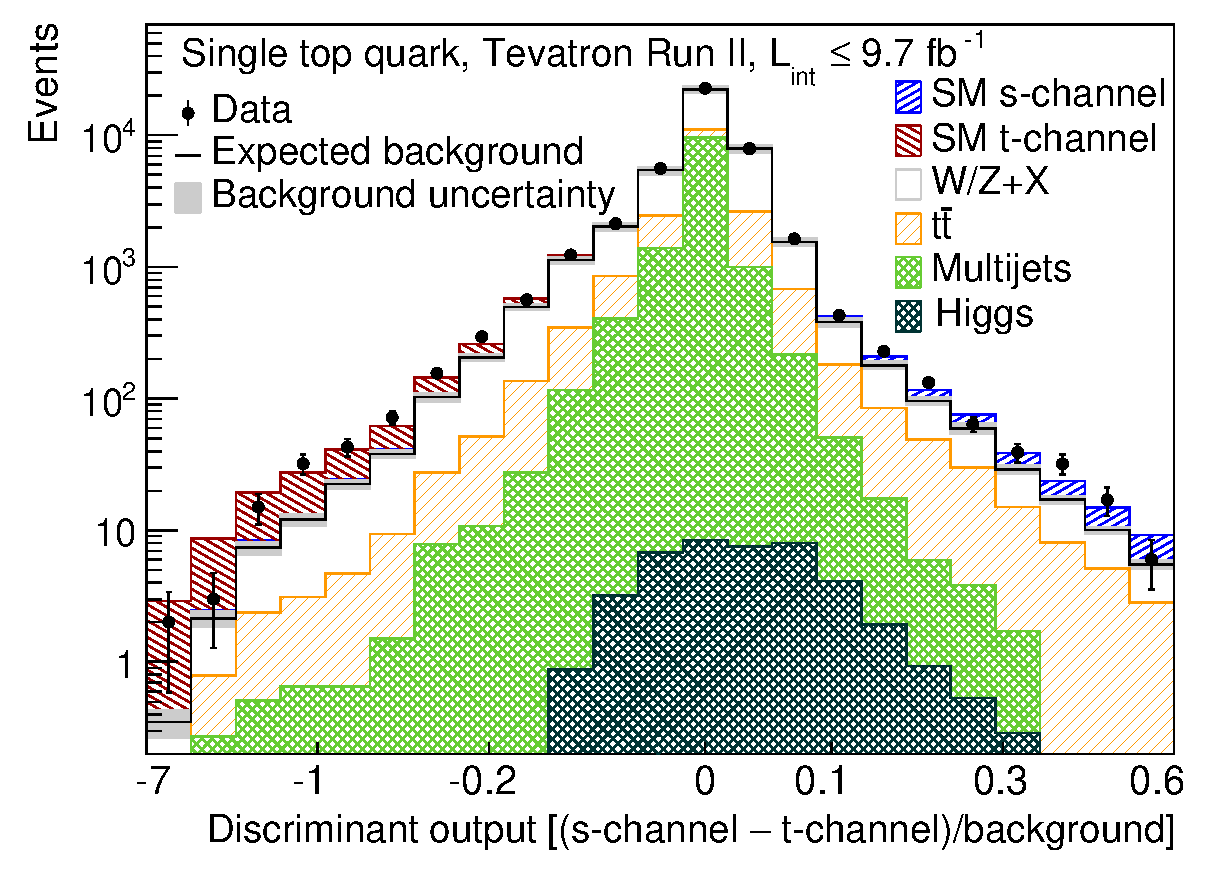
\includegraphics[width=0.48\textwidth]{fig01.eps}
\caption{Distribution of the mean discriminants for bins
  with similar ratios of ($s$-channel$-$$t$-channel) signals divided by
  background yields. The data,
  predicted SM $s$- and $t$-channel yields, and expected background
  are displayed. The total expected background (black solid line) is
  shown with its uncertainty (gray shaded band). A nonlinear scale is
  used on the abscissa to better display the range of the discriminant
  output values.}
\label{fig:TevtbtqbSubtrLog}
\end{center}
\end{figure}
%%%%%%%%%%%%%%%%%%%%%%%%%%%%%%%%%%%%%%%%%%%%%%%%%%%%

Figure~\ref{fig:tevposterior} presents the resulting 2D posterior
probability distribution as a function of $\sigma_t$ and $\sigma_s$.
%
%%%%%%%%%%%%%%%%%%%%%%%%%%%%%%%%%%%%%%%%%%%%%%%%%%%%
\begin{figure}[!h!tbp]
\begin{center}
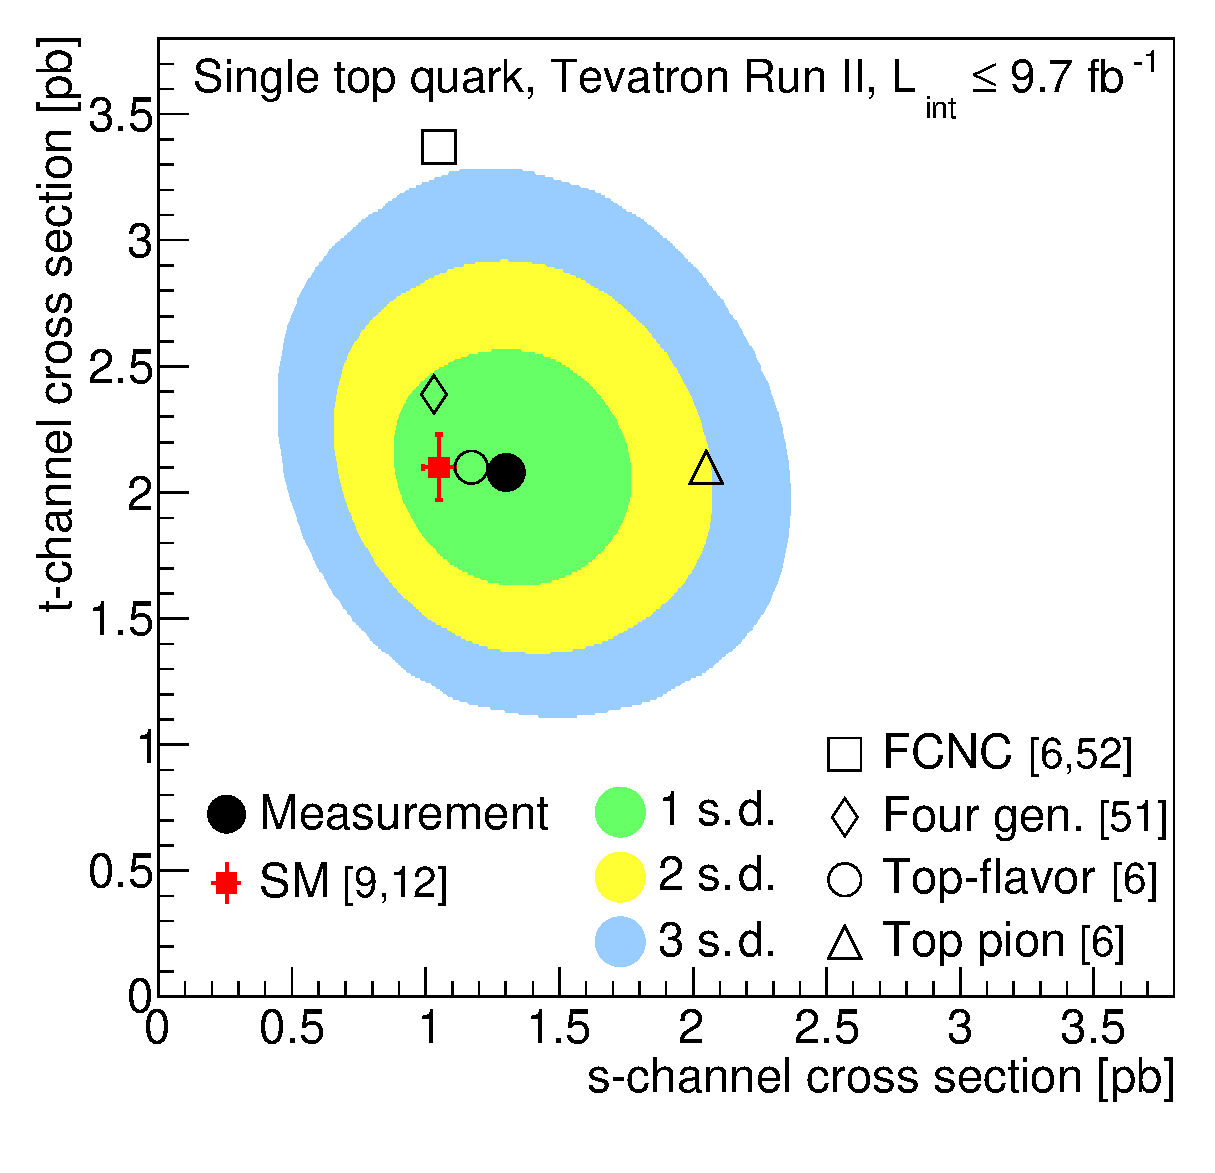
\includegraphics[width=0.48\textwidth]{fig02.eps}
\caption{Two-dimensional posterior probability as a function of
  $\sigma_t$ and $\sigma_s$ with one s.\ d. (68\% C.L.), two
  s.d. (95\% C.L.), and three s.\ d. (99.7\% C.L.) probability
  contours for the combination of the CDF and D0 analysis channels
  compared with the NLO+NNLL theoretical prediction of the
  SM~\cite{schannel-kidonakis,tchannel-kidonakis}. Several BSM
  predictions are shown, a model with four quark families with
  top-to-strange quark coupling $|V_{ts}| = 0.2$~\cite{FourthGen2}, a
  top-flavor model with new heavy bosons with mass $m_x = 
  1$\;TeV~\cite{Tait:2000sh}, a model of charged top pions with mass
  $m_{\pi^{\pm}} = 250$\;GeV~\cite{Tait:2000sh}, and a model with
  flavor-changing neutral currents with a 0.036 coupling
  $\kappa_u/\Lambda$ between up quark, top quark, and
  gluon~\cite{Tait:2000sh,d0-fcnc}.}
\label{fig:tevposterior}
\end{center}
\end{figure}
%%%%%%%%%%%%%%%%%%%%%%%%%%%%%%%%%%%%%%%%%%%%%%%%%%%%
%
The value and uncertainty in the individual cross sections are derived
through the 1D posterior probability functions obtained by integrating
the 2D posterior probability over the other variable. The most
probable value of $\sigma_t$ is $2.25 ^{+0.29}_{-0.31}$~pb. The
measurement of $\sigma_{s+t}$ is performed without making assumptions
on the ratio of $\sigma_s/\sigma_t$ by forming a 2D posterior
probability density distribution of $\sigma_{s+t}$ versus $\sigma_t$
and then integrating over all possible values of $\sigma_t$ to extract
the 1D estimate of $\sigma_{s+t}$. The combined cross section is
$\sigma_{s+t} = 3.30^{+0.52}_{-0.40}$~pb. The total expected
uncertainty on $\sigma_{s+t}$ is 13\%, the expected uncertainty
without considering systematic uncertainties is 8\%, and the
expected systematic uncertainty is 10\%. The systematic
uncertainty from the limited precision of top-quark mass measurements
is negligible~\cite{cdf-prd-2010,d0_schannel}. Figure~\ref{fig:tevposterior} 
also shows the expectation from several beyond the SM (BSM) models. 
Figure~\ref{fig:tevxsec} shows the
individual~\cite{cdf_channels,d0_schannel} and combined (this Letter)
measurements of the $t$- and ($s+t$)-channel cross sections including
previous measurements of the
individual~\cite{cdf_schannel,d0_schannel} and
combined~\cite{tev_schannel} $s$-channel cross sections. All
measurements are consistent with SM predictions.
%
%%%%%%%%%%%%%%%%%%%%%%%%%%%%%%%%%%%%%%%%%%%%%%%%%%%%
\begin{figure}[!h!tbp]
\begin{center}
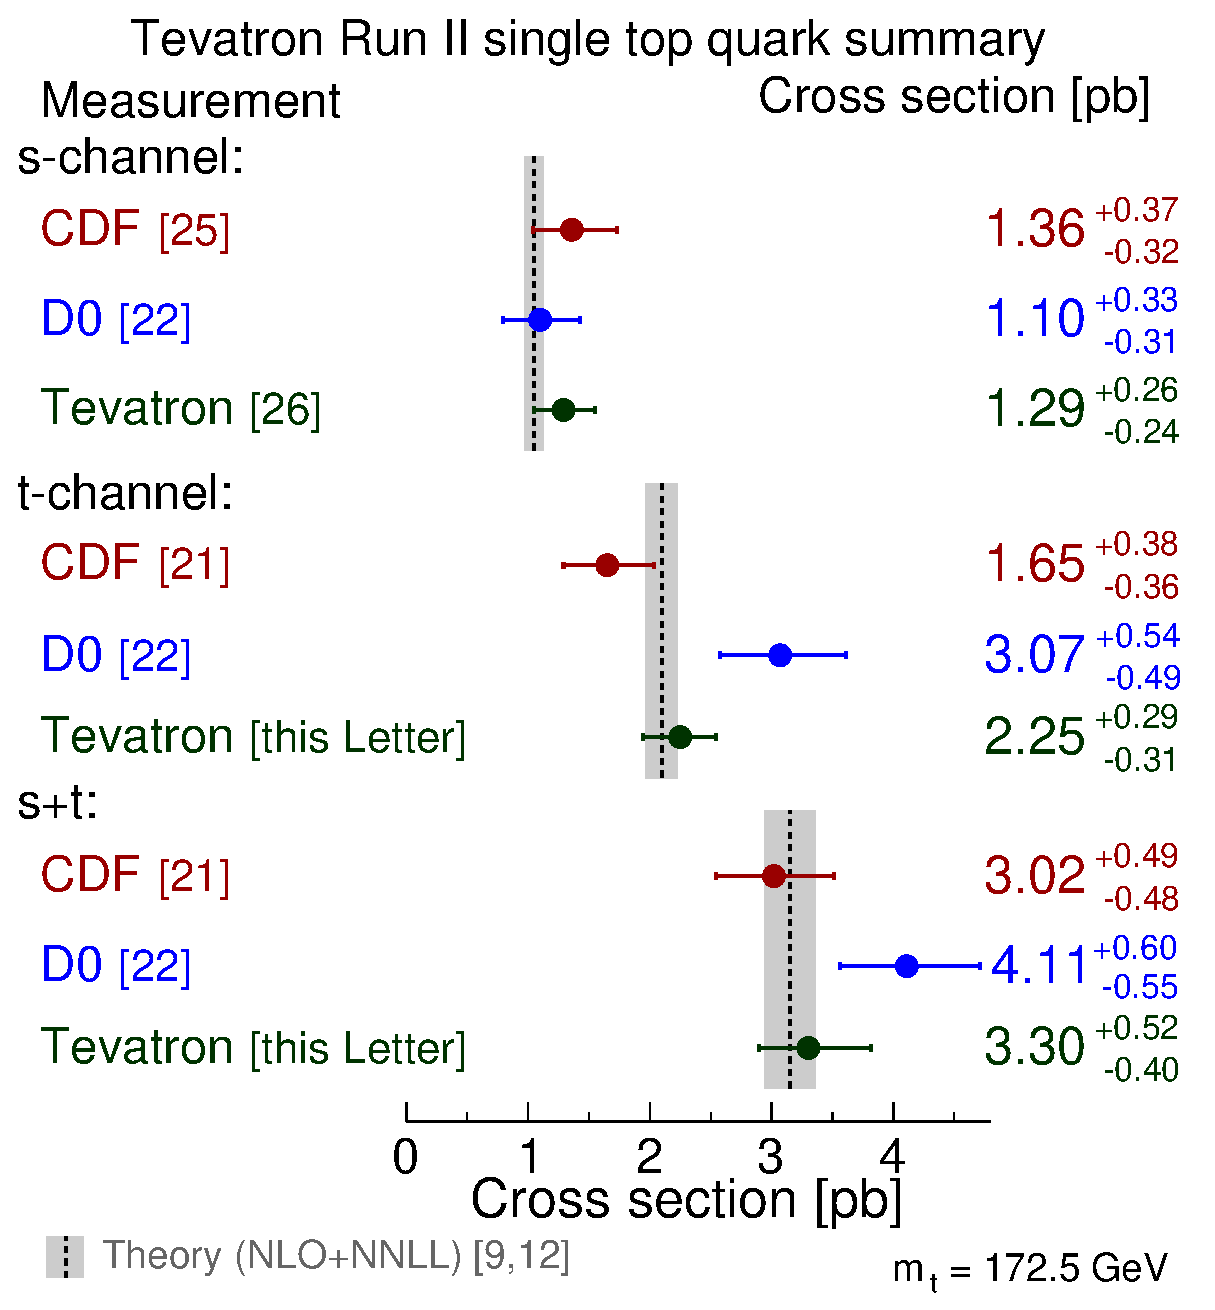
\includegraphics[width=0.48\textwidth]{fig03.eps}
\caption{Measured single-top-quark production cross
  sections from the CDF and D0 Collaborations in different production
  channels and the Tevatron combinations of these analyses compared
  with the NLO+NNLL theoretical
  prediction~\cite{schannel-kidonakis,tchannel-kidonakis}.}
\label{fig:tevxsec}
\end{center}
\end{figure}
%%%%%%%%%%%%%%%%%%%%%%%%%%%%%%%%%%%%%%%%%%%%%%%%%%%%

The SM single-top-quark production cross section is directly sensitive
to the square of the CKM matrix element
$V_{tb}$~\cite{tchannel-kidonakis,schannel-kidonakis}, thus  
providing a measurement of $|V_{tb}|$ without any assumption
on the number of quark families or the unitarity of the CKM
matrix~\cite{d0-prd-2008}.  
We extract $|V_{tb}|$ assuming that top quarks decay exclusively to
$Wb$ final states.  

We start with the multivariate discriminants for the $s$ and $t$
channels for each experiment and form a Bayesian posterior probability
density for $|V_{tb}|^2$ assuming a uniform-prior probability
distribution in the region $[0,\infty]$ corresponding to a uniform
prior density of the signal cross section. Additionally, the
uncertainties on the SM predictions for the $s$- and $t$-channel cross
sections~\cite{schannel-kidonakis,tchannel-kidonakis} are
considered. The resulting posterior probability distribution for
$|V_{tb}|^2$ is presented in Fig.~\ref{fig:TevVtb}. 
%
%%%%%%%%%%%%%%%%%%%%%%%%%%%%%%%%%%%%%%%%%%%%%%%%%%%%
\begin{figure}[!h!tbp]
\begin{center}
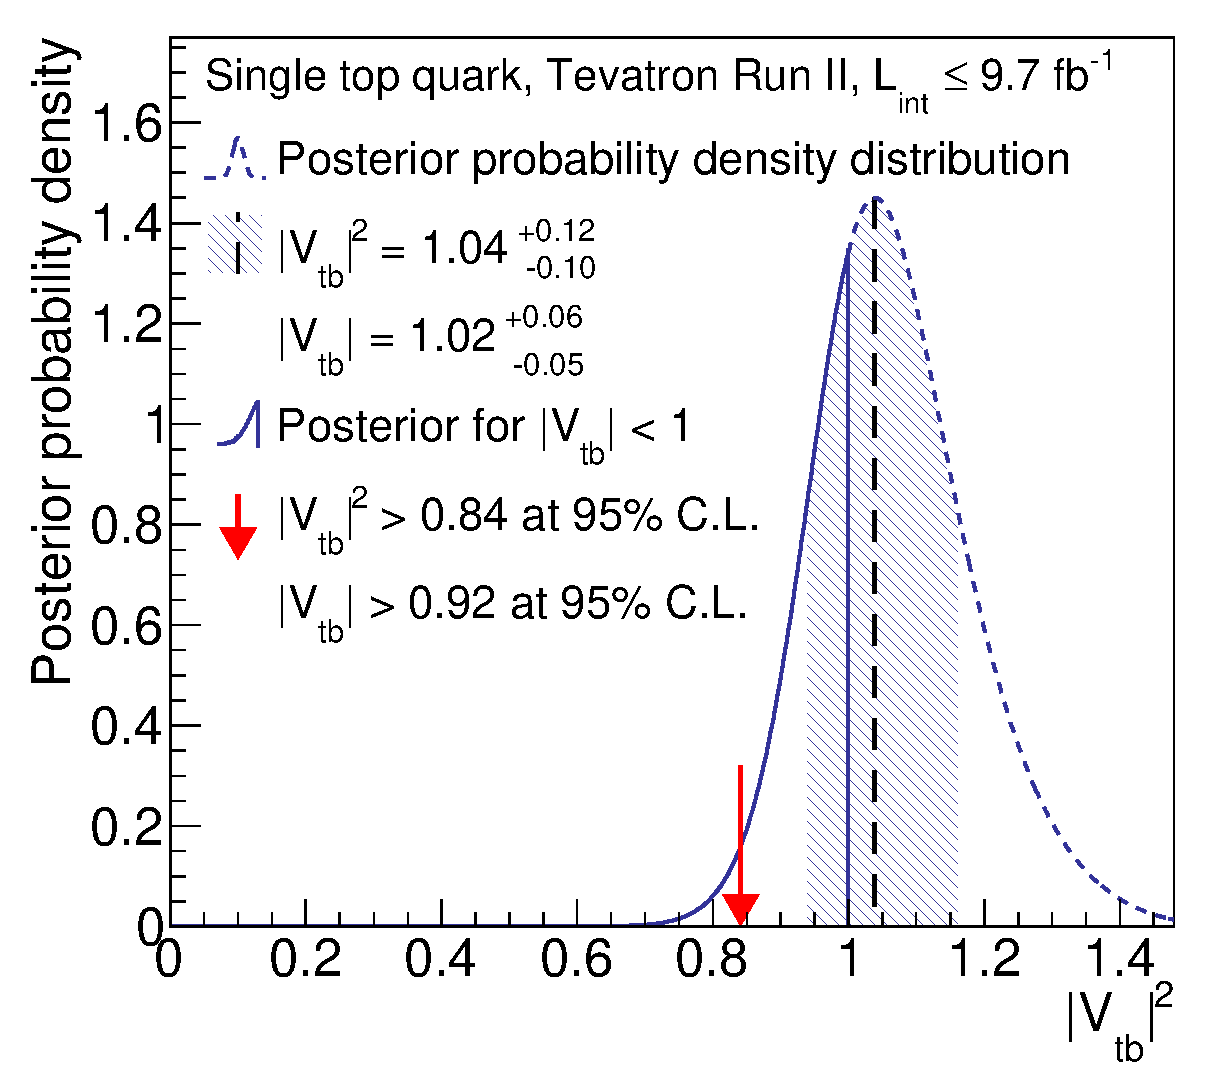
\includegraphics[width=0.48\textwidth]{fig04.eps}
\caption{Posterior probability distribution as a
  function of $|V_{tb}|^2$ for the combination of CDF and D0 analysis
  channels. The arrow indicates the allowed values of $|V_{tb}|^2$
  corresponding to the limit of $|V_{tb}| > 0.92$ at the $95\%$~C.L.} 
\label{fig:TevVtb}
\end{center}
\end{figure}
%%%%%%%%%%%%%%%%%%%%%%%%%%%%%%%%%%%%%%%%%%%%%%%%%%%%
%
We obtain $|V_{tb}| = 1.02^{+0.06}_{-0.05}$. If we restrict the prior
to the SM region [0,1], we extract a limit of $|V_{tb}| > 0.92$ at the
$95\%$~C.L.  



%%%%%%%%%%%%%%%%%%%%%%%%%%%
%% 
%% Summary
%% 
%%%%%%%%%%%%%%%%%%%%%%%%%%%


In summary, using $p\bar{p}$ collision samples corresponding to an
integrated luminosity of up to 9.7\;fb$^{-1}$ per experiment, we
report the final combination of single-top-quark production cross
sections from CDF and D0 measurements assuming $m_t=172.5$\;GeV. The
cross section for $t$-channel production is found to be  
\[\sigma_t = 2.25 ^{+0.29}_{-0.31}\;\rm pb .\] Without assuming the SM
value for the relative $s$- and $t$-channel contributions, the total
single-top-quark production cross section is \[\sigma_{s+t} =
3.30^{+0.52}_{-0.40}\;\rm pb.\] Together with the combined $s$-channel
cross section~\cite{tev_schannel}, this completes single-top-quark
cross-section measurements accessible at the Tevatron. All
measurements are consistent with SM
predictions~\cite{schannel-kidonakis,tchannel-kidonakis}. Finally, we
extract a direct limit on the CKM matrix element of $|V_{tb}| > 0.92$
at the $95\%$~C.L. As a result, there is no indication of sources of
new physics beyond the SM in the measured strength of the $Wtb$
coupling. 
 

%---------------------------------------------------------------------


%%%%%%%%%%%%%%%%%%%%%%%%%%%
\section*{Acknowledgments}
We thank the Fermilab staff and technical staffs of the participating
institutions for their vital contributions. We acknowledge support
from the Department of Energy and the National Science Foundation
(U.S.A.), the Australian Research Council (Australia), the National
Council for the Development of Science and Technology and the Carlos
Chagas Filho Foundation for the Support of Research in the State of
Rio de Janeiro (Brazil), the Natural Sciences and Engineering Research
Council (Canada), the China Academy of Sciences, the National Natural
Science Foundation of China, and the National Science Council of the
Republic of China (China), the Administrative Department of Science,
Technology and Innovation (Colombia), the Ministry of Education, Youth
and Sports (Czech Republic), the Academy of Finland, the Alternative
Energies and Atomic Energy Commission and the National Center for
Scientific Research/National Institute of Nuclear and Particle Physics
(France), the Bundesministerium f{\"u}r Bildung und Forschung (Federal
Ministry of Education and Research) and the Deutsche
Forschungsgemeinschaft (German Research Foundation) (Germany), the
Department of Atomic Energy and Department of Science and Technology
(India), the Science Foundation Ireland (Ireland), the National
Institute for Nuclear Physics (Italy), the Ministry of Education,
Culture, Sports, Science and Technology (Japan), the Korean World
Class University Program and the National Research Foundation of Korea
(Korea), the National Council of Science and Technology (Mexico), the
Foundation for Fundamental Research on Matter (Netherlands), the
Ministry of Education and Science of the Russian Federation, the
National Research Center ``Kurchatov Institute'' of the Russian
Federation, and the Russian Foundation for Basic Research (Russia),
the Slovak R\&D Agency (Slovakia), the Ministry of Science and
Innovation, and the Consolider-Ingenio 2010 Program (Spain), the
Swedish Research Council (Sweden), the Swiss National Science
Foundation (Switzerland), the Ministry of Education and Science of
Ukraine (Ukraine), the Science and Technology Facilities Council and
the The Royal Society (United Kingdom), the A.P. Sloan Foundation
(U.S.A.), and the European Union community Marie Curie Fellowship
Contract No. 302103.
%

%%%%%%%%%%%%%%%%%%%%%%%%%%%


%%%%%%%%%%%%%%%%%%%%%%%%%%%
\begin{thebibliography}{99}
%%%%%%%%%%%%%%%%%%%%%%%%%%%


\bibitem{top}
  C.~E.~Gerber and C.~Vellidis,
  %``Review of Tevatron Results: Top quark physics,''
  arXiv:1409.5038.

\bibitem{ttbar_combi}
  T.~A.~Aaltonen {\it et al.}  (CDF and D0 Collaborations),
  %``Combination of measurements of the top-quark pair production cross section from the Tevatron Collider,''
  Phys.\ Rev.\ D {\bf 89}, 072001 (2014).
  %[arXiv:1309.7570 [hep-ex]].

\bibitem{ckm} N.~Cabibbo,
  %``Unitary Symmetry and Leptonic Decays,''
  Phys.\ Rev.\ Lett.\  {\bf 10}, 531 (1963); \\
 M.~Kobayashi and T.~Maskawa,
  %``CP Violation In The Renormalizable Theory Of Weak Interaction,''
  Prog.\ Theor.\ Phys.\  {\bf 49}, 652 (1973).

\bibitem{FourthGen1} 
  M.~S.~Chanowitz,
  %``Bounding CKM Mixing with a Fourth Family,''
  Phys.\ Rev.\ D {\bf 79}, 113008 (2009).
  %[arXiv:0904.3570 [hep-ph]].

\bibitem{FourthGen2} 
  J.~Alwall, R.~Frederix, J.-M.~G{\'e}rard, A.~Giammanco, M.~Herquet, S.~Kalinin, E.~Kou, V.~Lemaitre, and F. Maltoni,
  %``Is V(tb) =~ 1?,''
  Eur.\ Phys.\ J.\ C {\bf 49}, 791 (2007).
  %[hep-ph/0607115].

\bibitem{Tait:2000sh}
  T.~M.~P.~Tait and C.-P.~Yuan,
  %``Single top quark production as a window to physics beyond the Standard
  %Model,''
  Phys.\ Rev.\  D {\bf 63}, 014018 (2000).
  %[arXiv:hep-ph/0007298].

\bibitem{singletop-willenbrock}
S.~S.~D.~Willenbrock and D.~A.~Dicus,
%''Production of Heavy Quarks from $W$ Gluon Fusion,''
Phys.\ Rev.\ D {\bf 34}, 155 (1986).

\bibitem{singletop-yuan}
C.-P.~Yuan,
%''A New Method to Detect a Heavy Top Quark at the Tevatron,''
Phys.\ Rev.\ D {\bf 41}, 42 (1990).

\bibitem{tchannel-kidonakis}
  N.~Kidonakis,
  %``Next-to-next-to-leading-order collinear and soft gluon corrections for t-channel single top quark production,''
  Phys.\ Rev.\ D {\bf 83}, 091503 (2011).
  %[arXiv:1103.2792 [hep-ph]].
  
\bibitem{singletop-cortese}
S.~Cortese and R.~Petronzio,
%''The Single Top Production Channel at Tevatron Energies,''
Phys.\ Lett.\ B {\bf 253}, 494 (1991).

%\cite{Tait:1999cf}
\bibitem{Wt-tait} 
  T.~M.~P.~Tait,
  %``The $t W^{-}$ mode of single top production,''
  Phys.\ Rev.\ D {\bf 61}, 034001 (1999).
%  [hep-ph/9909352].

\bibitem{schannel-kidonakis}
  N.~Kidonakis,
  %``NNLL resummation for s-channel single top quark production,''
  Phys.\ Rev.\ D {\bf 81}, 054028 (2010).
%  [arXiv:1001.5034 [hep-ph]].

\bibitem{topmasswa}
ATLAS, CDF, CMS and D0 Collaborations,
  %``First combination of Tevatron and LHC measurements of the top-quark mass,''
  arXiv:1403.4427.
 
\bibitem{pdg} 
K.~A.~Olive {\it et al.}  (Particle Data Group),
  %``Review of Particle Physics (RPP),''
  Chin.\ Phys.\ C {\bf 38}, 090001 (2014).

\bibitem{stop-obs-2009-cdf}
T.~Aaltonen {\it et al.} (CDF Collaboration),
%``Observation of Electroweak Single Top-Quark Production,''
Phys.\ Rev.\ Lett.\ {\bf 103}, 092002 (2009).

\bibitem{Aaltonen:2010fs}
  T.~Aaltonen {\it et al.}  (CDF Collaboration),
  %``Search for single top quark production in pbar $p$ collisions at $\sqrt{s}=1.96$ TeV in the missing transverse energy plus jets topology,''
  Phys.\ Rev.\ D {\bf 81} 072003 (2010).
%  [arXiv:1001.4577 [hep-ex]].

\bibitem{cdf-prd-2010} 
  T.~Aaltonen {\it et al.}  (CDF Collaboration),
  %``Observation of Single Top Quark Production and Measurement of |Vtb| with CDF,''
  Phys.\ Rev.\ D {\bf 82}, 112005 (2010).

\bibitem{stop-obs-2009-d0}
V.~M.~Abazov {\it et al.} (D0 Collaboration),
%``Observation of Single Top-Quark Production,''
Phys.\ Rev.\ Lett.\ {\bf 103}, 092001 (2009).

\bibitem{stop-2011-d0} 
  V.~M.~Abazov {\it et al.}  (D0 Collaboration),
  %``Measurements of single top quark production cross sections and $|V_{tb}|$ in $p\bar{p} collisions at $\sqrt{s}=1.96$ TeV,''
  Phys.\ Rev.\ D {\bf 84}, 112001 (2011).
  %[arXiv:1108.3091 [hep-ex]].

\bibitem{cdf_channels_7.5}
  T.~A.~Aaltonen {\it et al.}  (CDF Collaboration),
  %``Measurement of the Single Top Quark Production Cross Section and |Vtb| in Events with One Charged Lepton, Large Missing Transverse Energy, and Jets at CDF,''
Phys. Rev. Lett. {\bf 113}, 261804 (2014).
  %arXiv:hep-ex/1407.4031.

\bibitem{cdf_channels}
  T.~A.~Aaltonen {\it et al.}  (CDF Collaboration),
  %``Updated Measurement of the Single Top Quark Production Cross Section and $V{tb}$ in the Missing Transverse Energy Plus Jets Topology in $p\bar{p}$ Collisions at $\sqrt{s} = 1.96$ TeV,''
  arXiv:1410.4909 [Phys. Rev. Lett. (to be published)].

\bibitem{d0_schannel}
  V.~M.~Abazov {\it et al.}  (D0 Collaboration),
  %``Evidence for s-channel single top quark production in $p\bar{p}$ collisions at $\sqrt{s}$ = 1.96 TeV,''
  Phys.\ Lett.\ B {\bf 726}, 656 (2013).
%  [arXiv:1307.0731 [hep-ex]].

\bibitem{t-channel-new}
  V.~M.~Abazov {\it et al.}  (D0 Collaboration),
  %``Model-independent measurement of $t$-channel single top quark production in $p\bar{p}$ collisions at $\sqrt{s}=1.96$ TeV,''
  Phys.\ Lett.\ B {\bf 705}, 313 (2011).
  %[arXiv:1105.2788 [hep-ex]].

\bibitem{cdf_schannel}
  T.~A.~Aaltonen {\it et al.}  (CDF Collaboration),
  %``Evidence for $s$-channel Single-Top-Quark Production in Events with one Charged Lepton and two Jets at CDF,''
  Phys.\ Rev.\ Lett.\  {\bf 112}, 231804 (2014).
%  [arXiv:1402.0484 [hep-ex]].

\bibitem{cdf_schannel_MET}
  T.~A.~Aaltonen {\it et al.}  (CDF Collaboration),
  %``Search for $s$-channel Single Top Quark Production in the Missing Energy Plus Jets Sample using the Full CDF II Data Set,''
  Phys.\ Rev.\ Lett.\  {\bf 112}, 231805 (2014).
%  [arXiv:1402.3756 [hep-ex]].

\bibitem{tev_schannel}
  T.~A.~Aaltonen {\it et al.}  (CDF and D0 Collaborations),
  %``Observation of s-channel production of single top quarks at the Tevatron,''
  Phys.\ Rev.\ Lett.\  {\bf 112}, 231803 (2014).
%  [arXiv:1402.5126 [hep-ex]].

\bibitem{atlas-tchannel-1}
  G.~Aad {\it et al.}  (ATLAS Collaboration),
  %``Measurement of the $t$-channel single top-quark production cross section in $pp$ collisions at $\sqrt{s}=7$ TeV with the ATLAS detector,''
  Phys.\ Lett.\ B {\bf 717}, 330 (2012).
  %[arXiv:1205.3130 [hep-ex]].

\bibitem{atlas-tchannel-2} 
  G.~Aad {\it et al.}  (ATLAS Collaboration),
  %``Comprehensive measurements of $t$-channel single top-quark production cross sections at $\sqrt{s} = 7$ TeV with the ATLAS detector,''
Phys.\ Rev.\ D {\bf 90}, 112006 (2014).
  %arXiv:hep-ex/1406.7844.

\bibitem{cms-tchannel-1}  
  S.~Chatrchyan {\it et al.}  (CMS Collaboration),
  %``Measurement of the single-top-quark $t$-channel cross section in $pp$ collisions at $\sqrt{s}=7$ TeV,''
  J.\ High\ Energy\ Phys.\ {\bf 12}, 035 (2012).

\bibitem{cms-tchannel-2} 
  V.~Khachatryan {\it et al.}  (CMS Collaboration),
  %``Measurement of the t-channel single-top-quark production cross section and of the $\mid V_{tb} \mid$ CKM matrix element in pp collisions at $\sqrt{s}$= 8 TeV,''
   J.\ High\ Energy\ Phys.\ {\bf 06}, 090 (2014).
 % [arXiv:1403.7366 [hep-ex]].

\bibitem{atlas-tW}  
   G.~Aad {\it et al.}  (ATLAS Collaboration),
  %``Evidence for the associated production of a $W$ boson and a top quark in ATLAS at $\sqrt{s}=7$ TeV,''
  Phys.\ Lett.\ B {\bf 716}, 142 (2012).

\bibitem{cms-tW}
  S.~Chatrchyan {\it et al.}  (CMS Collaboration),
  %``Observation of the associated production of a single top quark and a W boson in pp collisions at sqrt(s) = 8 TeV,''
  Phys.\ Rev.\ Lett.\  {\bf 112}, 231802 (2014).
  %[arXiv:1401.2942 [hep-ex]].

\bibitem{CDFII} 
  D.~Acosta {\it et al.}  (CDF Collaboration),
  %``Measurement of the $J/\psi$ meson and $b-$hadron production cross sections in $p\bar{p}$ collisions at $\sqrt{s} = 1960$ GeV,''
  Phys.\ Rev.\ D {\bf 71}, 032001 (2005).
  %[hep-ex/0412071].

\bibitem{D0II} 
  V.~M.~Abazov {\it et al.}  (D0 Collaboration),
  %``The Upgraded D0 detector,''
  Nucl.\ Instrum.\ Methods Phys. Res., Sect. A {\bf 565}, 463 (2006).
  %[physics/0507191 [physics.ins-det]].

\bibitem{CDFbtag}
J. Freeman, T. Junk, M. Kirby, Y. Oksuzian, T. J. Phillips,
F. D. Snider, M. Trovato, J. Vizan, and W. M. Yao,
Nucl. Instrum. Meth. in Phys. Res.
 A {\bf 697}, 64 (2013).

\bibitem{D0btag}
  V.~M.~Abazov {\it et al.} (D0 Collaboration),
  %``b-Jet Identification in the D0 Experiment,''
  Nucl. Instrum. Methods Phys. Res., Sect. A {\bf 620}, 490 (2010);
  %Improved b-Quark Jet Identification at the D0 Experiment to be submitted to NIM. 
  V.~M.~Abazov {\it et al.}  (D0 Collaboration),
  %``Improved $b$ quark jet identification at the D0 experiment,''
  Nucl. Instrum. Methods Phys. Res., Sect. A {\bf 763}, 290 (2014).
  %arXiv:1312.7623.

\bibitem{cdf_matrix_method}
  T.~Aaltonen {\it et al.}  [CDF Collaboration],
  %``Updated search for the standard model Higgs boson in events with jets and missing transverse energy using the full CDF data set,''
  Phys.\ Rev.\ D {\bf 87}, 052008 (2013).

\bibitem{d0-prd-2008}
V.~M.~Abazov {\it et al.} (D0 Collaboration),
%``Evidence for Production of Single Top Quarks,''
Phys.\ Rev.\ D\ {\bf 78}, 012005 (2008).

\bibitem{POWHEG2009} 
  S.~Alioli, P.~Nason, C.~Oleari, and E.~Re,
  %``NLO single-top production matched with shower in POWHEG: s- and t-channel contributions,''
  J.\ High Energy Phys. {\bf 09}, 111 (2009).
  %[Erratum-ibid.\  {\bf 1002}, 011 (2010)]
  %[arXiv:0907.4076 [hep-ph]].

\bibitem{singletop-mcgen}
  E.~E.~Boos, V. E. Bunichev,  L. V. Dudko,  V. I. Savrin, and  V. V. Sherstnev,
  %''Method for Simulating Electroweak Top-Quark Production Events in
  %the NLO Approximation: SingleTop Event Generator,''
  Phys.\ Atom.\ Nucl.\ {\bf 69}, 1317 (2006). We use {\singletop}
  version 4.2p1.

\bibitem{singletop-xsec-sullivan}
  Z.~Sullivan, Phys.\ Rev.\ D~{\bf 70}, 114012 (2004).

\bibitem{Campbell:2009ss}
  J.~M.~Campbell, R.~Frederix, F.~Maltoni, and F.~Tramontano,
  %``$t^-$ channel single-top production at hadron colliders,''
  Phys.\ Rev.\ Lett.\ {\bf 102}, 182003 (2009). 
  %arXiv:0903.0005 [hep-ph].

\bibitem{alpgen}
  M.~L.~Mangano, M.~Moretti, F.~Piccinini, R.~Pittau, and A.D.~Polosa,
  %``ALPGEN, a Generator for Hard Multiparton Processes in Hadronic
  %Collisions,''
  J.\ High Energy Phys. {\bf 07}, 001 (2003). We use {\alpgen} version 2.11.

\bibitem{pythia}
  T.~Sj\"{o}strand, S.~Mrenna, and P.~Skands,
  %``PYTHIA 6.4 Physics and Manual,''
  J.\ High Energy Phys. {\bf 05}, 026 (2006). We use {\pythia} version 6.409.

\bibitem{MLM}
M.~L.~Mangano, M.~Moretti, and R.~Pittau, 
%Multijet matrix elements and shower evolution in hadronic collisions:
%Wbbar + n jets as a case study, 
Nucl.\ Phys.\ B {\bf 632}, 343 (2002).

\bibitem{atlas-higgs-mass}
  G.~Aad {\it et al.}  (ATLAS Collaboration),
  %``Measurement of the Higgs boson mass from the $H\rightarrow \gamma\gamma$ and $H \rightarrow ZZ^{*} \rightarrow 4\ell$ channels with the ATLAS detector using 25 fb$^{-1}$ of $pp$ collision data,''
  Phys.\ Rev.\ D {\bf 90}, 052004 (2014).
%  [arXiv:1406.3827 [hep-ex]].

\bibitem{cms-higgs-mass1} 
  V.~Khachatryan {\it et al.}  [CMS Collaboration],
  %``Observation of the diphoton decay of the Higgs boson and measurement of its properties,''
  Eur.\ Phys.\ J.\ C {\bf 74}, 3076 (2014).
%  [arXiv:1407.0558 [hep-ex]].

%\cite{Chatrchyan:2013mxa}
\bibitem{cms-higgs-mass2} 
  S.~Chatrchyan {\it et al.}  (CMS Collaboration),
  %``Measurement of the properties of a Higgs boson in the four-lepton final state,''
  Phys.\ Rev.\ D {\bf 89}, 092007 (2014);
%  [arXiv:1312.5353 [hep-ex]].

  G.~Aad {\it et al.}  (ATLAS Collaboration),
  %``Observation of a new particle in the search for the Standard Model Higgs boson with the ATLAS detector at the LHC,''
  Phys.\ Lett.\ B {\bf 716}, 1 (2012).
%  [arXiv:1207.7214 [hep-ex]].

\bibitem{geant}
  R.~Brun and F.~Carminati,
  %''GEANT: Detector Description and Simulation Tool,''
  CERN Program Library Long Writeup, Report No. W5013, 1993.

\bibitem{ttbar-xsec}
  S.~Moch and P.~Uwer,
  Phys.\ Rev.\ D {\bf 78}, 034003 (2008). 
  The top-quark-pair production cross section is $7.46 \pm 0.75$~pb
  ($m_t=172.5$~GeV). 

\bibitem{mcfm}
  R.~K.~Ellis,
  %''An Update on the Next-to-Leading Order Monte Carlo MCFM,''
  Nucl.\ Phys.\ Proc.\ Suppl.\ {\bf 160}, 170 (2006). We use {\mcfm}
  version 5.1.

\bibitem{higgs-xsec} 
  J.~Baglio and A.~Djouadi,
  %``Predictions for Higgs production at the Tevatron and the associated uncertainties,''
  J.\ High Energy Phys. {\bf 10}, 064 (2010);
 %  [arXiv:1003.4266 [hep-ph], arXiv:1009.1363 [hep-ph]].
  %%CITATION = ARXIV:1003.4266;%%
  G.~Ferrera, M.~Grazzini, and F.~Tramontano,
  %``Associated WH production at hadron colliders: a fully exclusive QCD calculation at NNLO,''
  Phys.\ Rev.\ Lett.\  {\bf 107}, 152003 (2011).
%   [arXiv:1107.1164 [hep-ph]].

\bibitem{bayes-limits}
  I.~Bertram {\it et al.}, FERMILAB-TM-2104 (2000).

\bibitem{d0-fcnc}
V.~M.~Abazov {\it et al.} (D0 Collaboration),
%``Search for production of single top quarks via flavor-changing neutral currents at the Tevatron,''
Phys.\ Rev.\ Lett.\ {\bf 99}, 191802 (2007).



\end{thebibliography}

\end{document}


%---------------------------------------------------------------------
%---------------------------------------------------------------------

